\documentclass[french,10pt,dvipsnames,table]{beamer}%,handout,ignorenonframetext
\mode<presentation> {
  \usetheme{Boadilla}%Boadilla Madrid
 \usecolortheme{beaver} %crane
  %\setbeamertemplate{navigation symbols}{}
  }
\setbeamercovered{transparent}
\mode<article>{\usepackage{fullpage}}
\usepackage{babel}
\usepackage{ae,lmodern}
\usepackage[utf8]{inputenc}
\usepackage[T1]{fontenc}
\usepackage{url}
\usepackage{xcolor}
\usepackage{arydshln}
\usepackage{multirow}
\usepackage{tikz}
\usepackage{ulem}
\usepackage{cancel}
\usepackage{amssymb}
\usepackage[nolinks]{qrcode}

% URLs des QR codes — à mettre à jour
\newcommand{\urlSujet}{https://gitlab.univ-nantes.fr/iut.info1.dev.objets/sae201/sae201.2026}
\newcommand{\urlMattermost}{https://mattermost.univ-nantes.fr/signup_user_complete/?id=kz3jbup9stytdxbarm5x6u7tzh&md=link&sbr=su}


\title[]{SAE 2.01 : développement d'une application}
\subtitle{Le jeu de cartes Flip7}
\author[A. Lanoix]{Arnaud Lanoix Brauer\\ \scriptsize{\tt Arnaud.Lanoix@univ-nantes.fr}}
\institute[Dépt. Info]{
  
\includegraphics[height=2.5cm]{fig/iut.png} \\  

\includegraphics[height=1.3cm]{fig/logo_iut_pole_techno_univ_2022.png}}
\date[]{}
\logo{
\includegraphics[height=.9cm]{fig/logo_iut_2022.png}}

\makeatletter
\define@key{beamerframe}{wide}[10pt]{%
  \def\beamer@cramped{\itemsep #1\topsep0.5pt\relax}}
\makeatother
\begin{document}


\begin{frame}[plain]
  \titlepage
\end{frame}


% ---- Contexte SAE ----
\begin{frame}{SAE 2.01}
  \begin{columns}
    \begin{column}{0.72\textwidth}
      \begin{block}{Développement d'une application}
        \begin{itemize}
          \item SAE commune aux ressources \textbf{dev.objets}, \textbf{IHM} et \textbf{Qualité/tests}
          \item Équipes de \textbf{4 à 5 développeur.se.s}
          \item Travail \textbf{obligatoirement} à l'IUT durant les semaines S24, S25 et S26\\
                + temps personnel
        \end{itemize}
      \end{block}
      \begin{exampleblock}{Enseignant.e.s impliqué.e.s}
        C. Jacquin \quad E. Bigeon \quad J.-M. Mottu \quad A. Lanoix Brauer
      \end{exampleblock}
    \end{column}
    \begin{column}{0.25\textwidth}
      \centering
      \qrcode[height=2.2cm]{\urlSujet}\\[3pt]
      \scriptsize Sujet détaillé
    \end{column}
  \end{columns}
\end{frame}

% ---- Contexte Flip7 ----
\begin{frame}{Le jeu Flip7\textcopyright{}}
  \begin{columns}
    \begin{column}{0.6\textwidth}
      \begin{block}{Un jeu de cartes}
        \begin{itemize}
          \item Jeu édité par \textbf{Catch Up Games}
          \item But : collecter des cartes numérotées \textbf{0 à 12}\\
                sans doublon, pour marquer un maximum de points
          \item Risque de \textbf{doublon} (score nul)
          \item Des cartes \textbf{bonus} augmentent les points      
          \item Des cartes \textbf{spéciales} pimentent la partie\\
                (Stop, 2ndeChance ou  3 à la suite)
        \end{itemize}
      \end{block}
      \smallskip
      \url{https://flip-7.com}
    \end{column}
    \begin{column}{0.38\textwidth}
      \begin{center}
        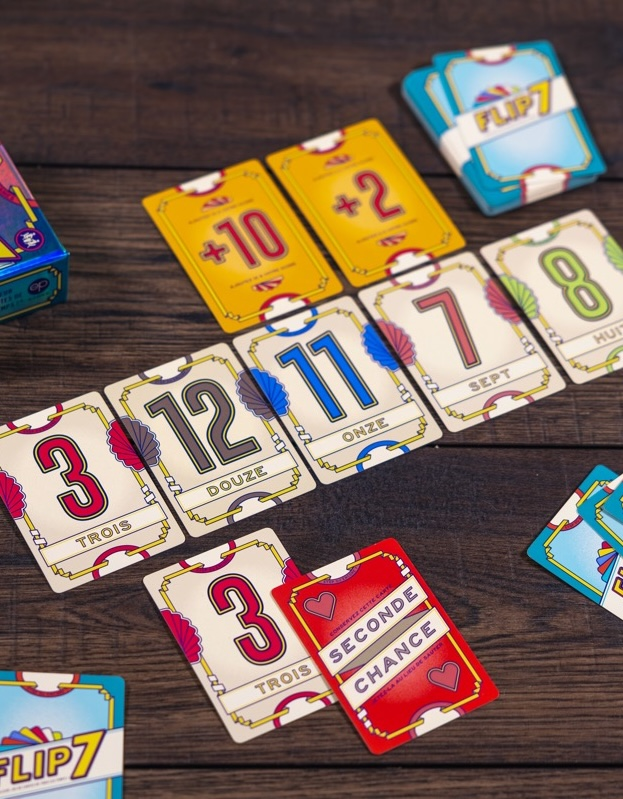
\includegraphics[width=\textwidth]{fig/flip7.jpg}
      \end{center}
    \end{column}
  \end{columns}
\end{frame}

% ---- 3 étapes ----
\begin{frame}{Les 3 grandes étapes}
  \begin{columns}
    \begin{column}{0.72\textwidth}
      \begin{enumerate}
        \item \textbf{Analyse et spécifications} du jeu Flip7
        \item \textbf{Conception et tests} d'une librairie implémentant la mécanique de jeu : \texttt{iut.info1.flip7-1.3.jar}
        \item \textbf{Développement} d'une application graphique \textbf{Kotlin/JavaFX} utilisant la librairie fournie
      \end{enumerate}
      \bigskip
      \begin{exampleblock}<2->{Gestion de projets / livrables}
        Exclusivement via \textbf{Gitlab} - dépôts bientôt créés
      \end{exampleblock}
      \bigskip
      \begin{block}<3>{Communication}
        Exclusivement via \textbf{Mattermost} (connexion GitLab) — pas d'emails ni de MP
      \end{block}

    \end{column}
    \begin{column}{0.25\textwidth}
      \centering
      \qrcode[height=2.2cm]{\urlMattermost}\\[3pt]
      \scriptsize Mattermost dédié
    \end{column}
  \end{columns}
\end{frame}

% ---- Calendrier ----
\begin{frame}{Calendrier des livraisons}
  \begin{center}
  \footnotesize
  \begin{tabular}{lll}
    \hline
    \textbf{Date} & \textbf{Heure} & \textbf{Livrable / Évaluation} \\
    \hline
    Jeudi 11/06    & 18h00          & Documents d'Analyse/spécifications \\
    Mercredi 17/06 & 18h00          & Conception des tests + code des tests \\
    Jeu. 18 / Ven. 19/06 & à définir & Revue de tests équipe/équipe \\
    Vendredi 19/06 & 18h00          & Maquette de l'application \\
    Jeudi 25/06    & 12h30          & Code fonctionnel de l'application JavaFX \\
    Jeu. 25 / Ven. 26/06 & à définir & Évaluation code/projet équipe/équipe \\
    Jeudi 25/06    & après-midi     & Revue de code par les pairs \\
    Vendredi 26/06 & 13h30 – 15h   & \textbf{TEST MACHINE FINAL} \\
    \hline
  \end{tabular}
  \end{center}
  \bigskip
  \begin{alertblock}<2>{Gitlab}
    Rendus des livrables sur votre dépôt Gitlab, \textbf{exclusivement}
  \end{alertblock}
\end{frame}

% ---- Tâche 1 : Analyse UML ----
\begin{frame}{Tâche 1 — Analyse et spécifications}
    \begin{enumerate}
      \item \textbf{Diagramme niveau Analyse} — description du jeu tel qu'il est, sans choix techniques
      \item \textbf{Diagramme niveau Conception détaillée} — raffinement intégrant Kotlin/JavaFX
    \end{enumerate}
 
  \begin{alertblock}<2->{Format PlantUML}
    \textbf{obligatoire} 
  \end{alertblock}
  \begin{exampleblock}<3>{Livrables sur votre dépot Gitlab}
    \begin{itemize}
      \item \texttt{rapport.md} — rapport décrivant vos choix d'analyse et de conception (au format Markdown \textbf{obligatoire})
      \item \texttt{analyse.puml} + \texttt{analyse.png} : diagramme d'analyse
      \item \texttt{detaille.puml} + \texttt{detaille.png} : diagramme de conception détaillée
    \end{itemize}
  \end{exampleblock}
  \textbf{Deadline :} jeudi 11/06 à 18h00
\end{frame}

% ---- Tâche 2 & 3 ----
\begin{frame}{Tâches 2 et 3 détaillées ultérieurement}
  \begin{block}{Tâche 2 — Tests d'une librairie fournies}
    \begin{itemize}
      \item Analyse et conception des tests
      \item Implémentation des tests 
      \item \textbf{Deadline :} mercredi 17/06 à 18h00
      \item Revue de tests avec un enseignant
    \end{itemize}
  \end{block}
  \begin{block}<2->{Tâche 3 — Application Kotlin/JavaFX}
    \begin{itemize}
      \item Maquettes de l'application (\textbf{Deadline :} 19/06 à 18h00)
      \item Code fonctionnel utilisant la librairie fournie (\textbf{Deadline :} 25/06 à 12h30)
      \item Revue de projet avec un enseignant
      \item Revue de code par les pairs
    \end{itemize}
  \end{block}
  \begin{alertblock}<3>{Rappel}
    Ne pas commencer à coder avant d'avoir réalisé les tâches précédentes.
  \end{alertblock}
\end{frame}

% ---- IA ----
\begin{frame}{À propos de l'usage de l'IA}
  \begin{alertblock}{Usage toléré mais déclaration obligatoire}
    \begin{itemize}
      \item Indiquer \textbf{quel outil} et \textbf{pour quel usage}
      \item Toute utilisation non déclarée $\Rightarrow$ \textbf{note 0}
      \item Vous devez être capables d'\textbf{expliquer et défendre} tout ce qui a été produit avec l'aide d'une IA
    \end{itemize}
  \end{alertblock}
  \bigskip
  L'objectif pédagogique est de \textbf{vous} faire mettre en application ce qui vous a été enseigné — pas à une IA.
\end{frame}

\end{document}
